\documentclass[UTF8,a4paper,12pt]{article}
\usepackage[top=2cm,bottom=2cm,left=2cm,right=2cm]{geometry}
\usepackage{algorithm}
\usepackage{algorithmicx}
\usepackage{algpseudocode}
\usepackage{amsmath}
\usepackage{tikz}

\usepackage{CJK}
\usepackage{amsmath,bm}
\usepackage{indentfirst}
\setlength{\parindent}{2em}
\floatname{algorithm}{PROBLEM}
\renewcommand{\algorithmicrequire}{INPUT:}
\renewcommand{\algorithmicensure}{OUTPUT:}

%\begin{CJK}{UTF8}{gkai}
\title{091M4041H - Assignment Five\\NetFlow}
\date{\today}
\author{张   帅\\201828018670119\\网络空间安全学院, UCAS}

%\end{CJK}


%\begin{CJK}{UTF8}{gkai}
%	你好,世界
%\end{CJK}


\begin{document}
	\begin{CJK}{UTF8}{gkai}
		\maketitle
		
	\newpage
	\section{Load balance}
	\subsection{题目描述}
		You have some different computers and jobs. For each job, it can only be done on one of two specified computers. The load of a computer is the number of jobs which have been done on the computer. Give the number of jobs and two computer ID for each job. You task is to minimize the max load.
	\subsection{解题思路}	
	
		假设有n个任务和m台计算机:
		
		每个任务$ J_i $可以由2台特定的电脑$ P_k、P_l $执行,因此我们可以建立一个超级源点$ S $,它指向m个jobs,capacity设置为1,流为1时,表示该job被执行;然后将每个任务$ J_i $与其2台特定的电脑$ P_k、P_l $建立有向边,capacity设置为1,流为1时,表示该边上的任务由该边所指向的电脑执行,该电脑负载加1;然后建立超级汇点$ T $,所有电脑指向该汇点,每条边capacit的值都一样,设为$ max_load $,表示电脑的最大运行负载,但需要动态设定。
		
		下面就是确定指向汇点的$ max_load $大小:题目要求我们要最小化最大负载的值,可以使用二分法来寻找最优的值。由题意知,一台电脑的最大负载发生在所有任务都在该电脑上执行,即负载为m,所以$ max_load $的取值范围[0,m],且为整数。这样利用二分法,执行$ log(m) $次最大流算法即可求出最优的值。
		
		建图如下:

	\begin{figure}[htb]
	\centering
	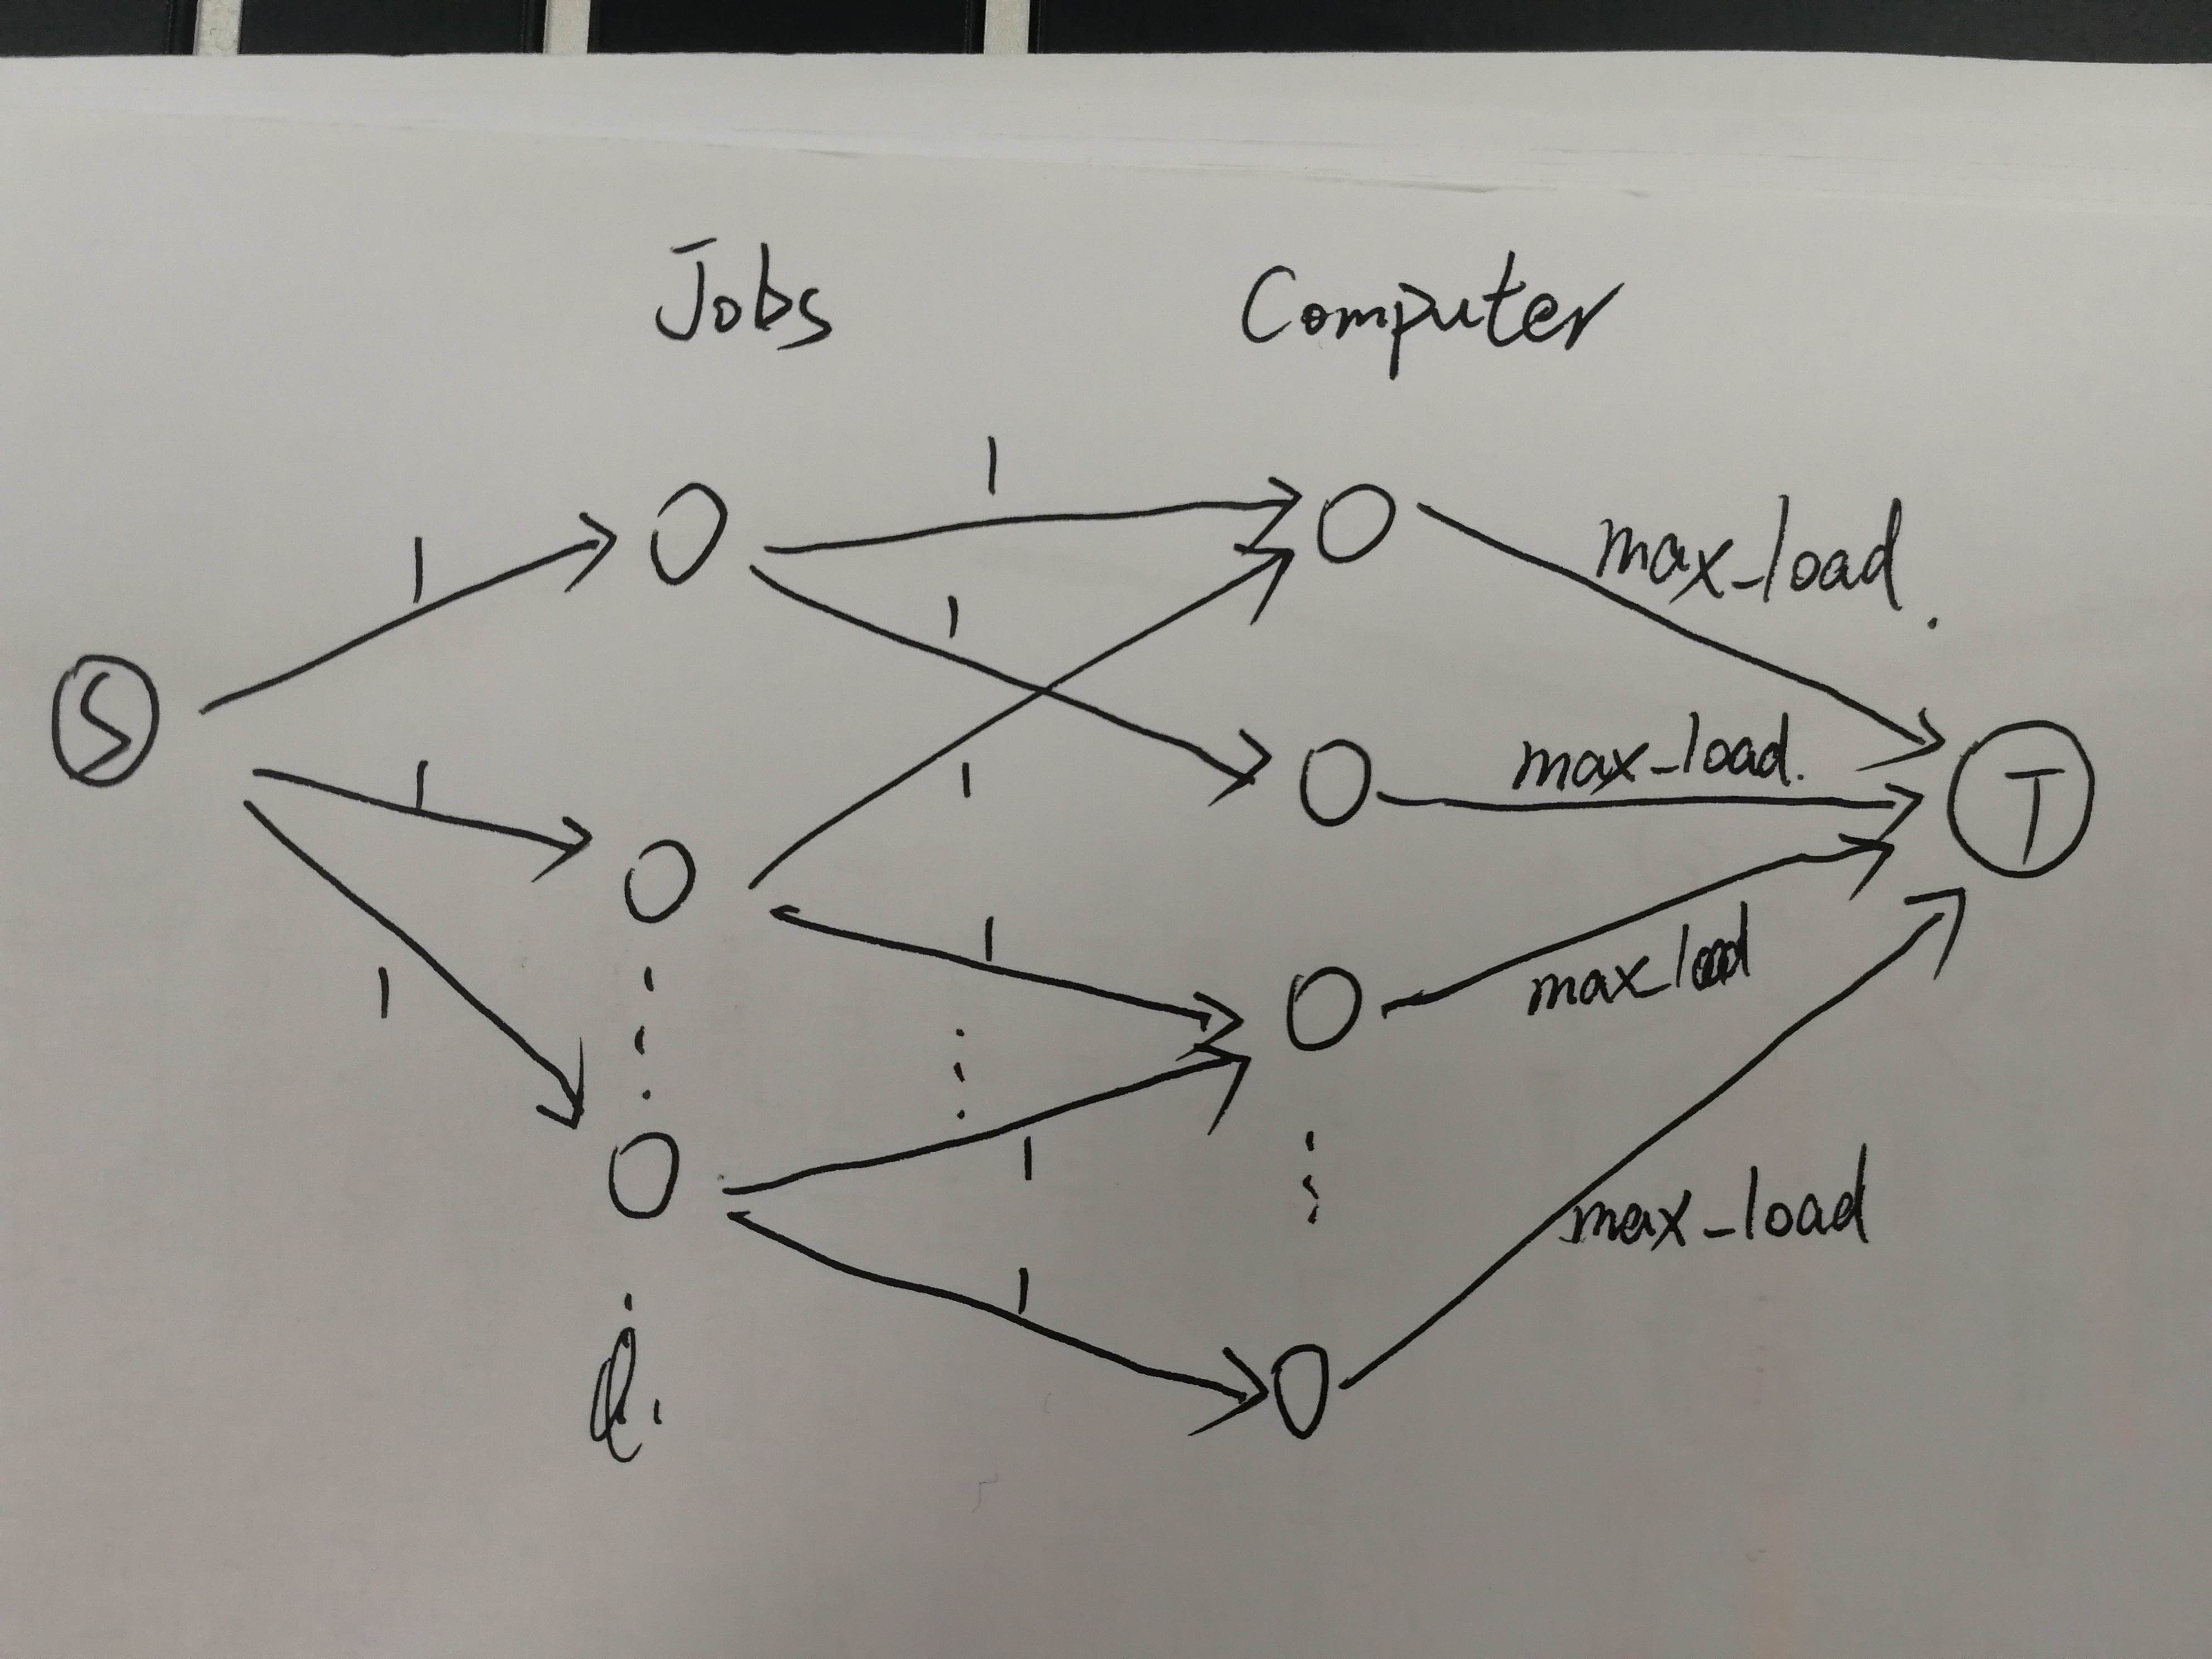
\includegraphics[scale=.1]{./1.jpg}
	\caption{Load balance}
\end{figure}
	
	\subsection{伪代码}
	
	\begin{algorithm}[htb]
		\caption{Load balance}
		\begin{algorithmic}[1]
			\Require a directed graph G associated with a job and a computer
			\Ensure Minimum load of the computer
			\Function{MinimumLoad}{G}
			\State create super nodes $S,T$
			\State $ N = \#job$
			\State $ r = N $
			\State $ l = 0 $
			\State $ max\_load = 0 $
			\State 使超级源点S指向所有的jobs,capacity设置为1;图G中的有向边的capacity都设置为1;所有主机指向超级汇点T,capacity暂时设置为r;构造出一个网络流 $ G' $
			\While{$ l>=num\_jobs $}
				\State $ mid = (l+r)/2 $
				\State 更新所有主机指向超级汇点的capacity,设置为mid;
				\State $f=Dinic(G')$执行Dinic算法,求出最大流f
				\If{$f==M$}
					\State $l = mid+1$
					\State $max\_load = mid$
				\Else
					\State $r = mid-1$
				\EndIf
			\EndWhile
			
			\State \Return $max\_load$
			\EndFunction	
		\end{algorithmic}
	\end{algorithm}
	
	\subsection{正确性证明}
		首先,从以上的表述中可以看到,我们动态设置了所有主机指向超级汇点的capacity max\_load,max\_load为各个主机到超级汇点T的容量上限,换句话说,主机的最大负载不能超过max\_load。另外我们设定超级源点到作业的capacity均为1,每个作业到其特定的两个主机的capacity也为1,这就保证每个工作只能运行在特定的两个主机的其中一个。然后我们运行最大流算法得出一个最大流f,如果f不等于作业数N,说明设置的max\_load不可行,需要增大;反之可行,可继续减小已测试是否有更小的设定。所以算法可行。
		
	\subsection{复杂度分析}
		假设有n个任务和m台计算机:
		那么边的数目$ M=m+n+2*n=3n+m $,节点数目$ N=1+m+n+1=m+n+2 $,运行Dinic算法的时间复杂度为$ O(N^2M) $,使用二分法共需迭代$ \log_{2}n $次,所以总的复杂度为:
		
		\begin{equation*}
			\begin{split}
			O(N^{2}M\log_{2}n)
			\end{split}
		\end{equation*}
		其中:$ N=1+m+n+1=m+n+2 $、$ M=m+n+2*n=3n+m $

	\newpage
	\section{Matrix}
	\subsection{题目描述}
	For a matrix filled with 0 and 1, you know the sum of every row and column. You are asked to give such a matrix which satisfys the conditions.
	
	\subsection{解题思路}
	假设有n行m列。
	
	我们添加超级源点S和超级汇点T,将每一行的和与每一列的和作为结点,行的和的结点与列的和的结点全连接,并设它们的capacity为1;然后让S与行和结点相连,capacity为每一行的和,列和结点与超级汇点T相连,capacity为每一列的和,对此网络流运行最大流算法,即可找到相应的矩阵。
	
		\begin{figure}[htb]
		\centering
		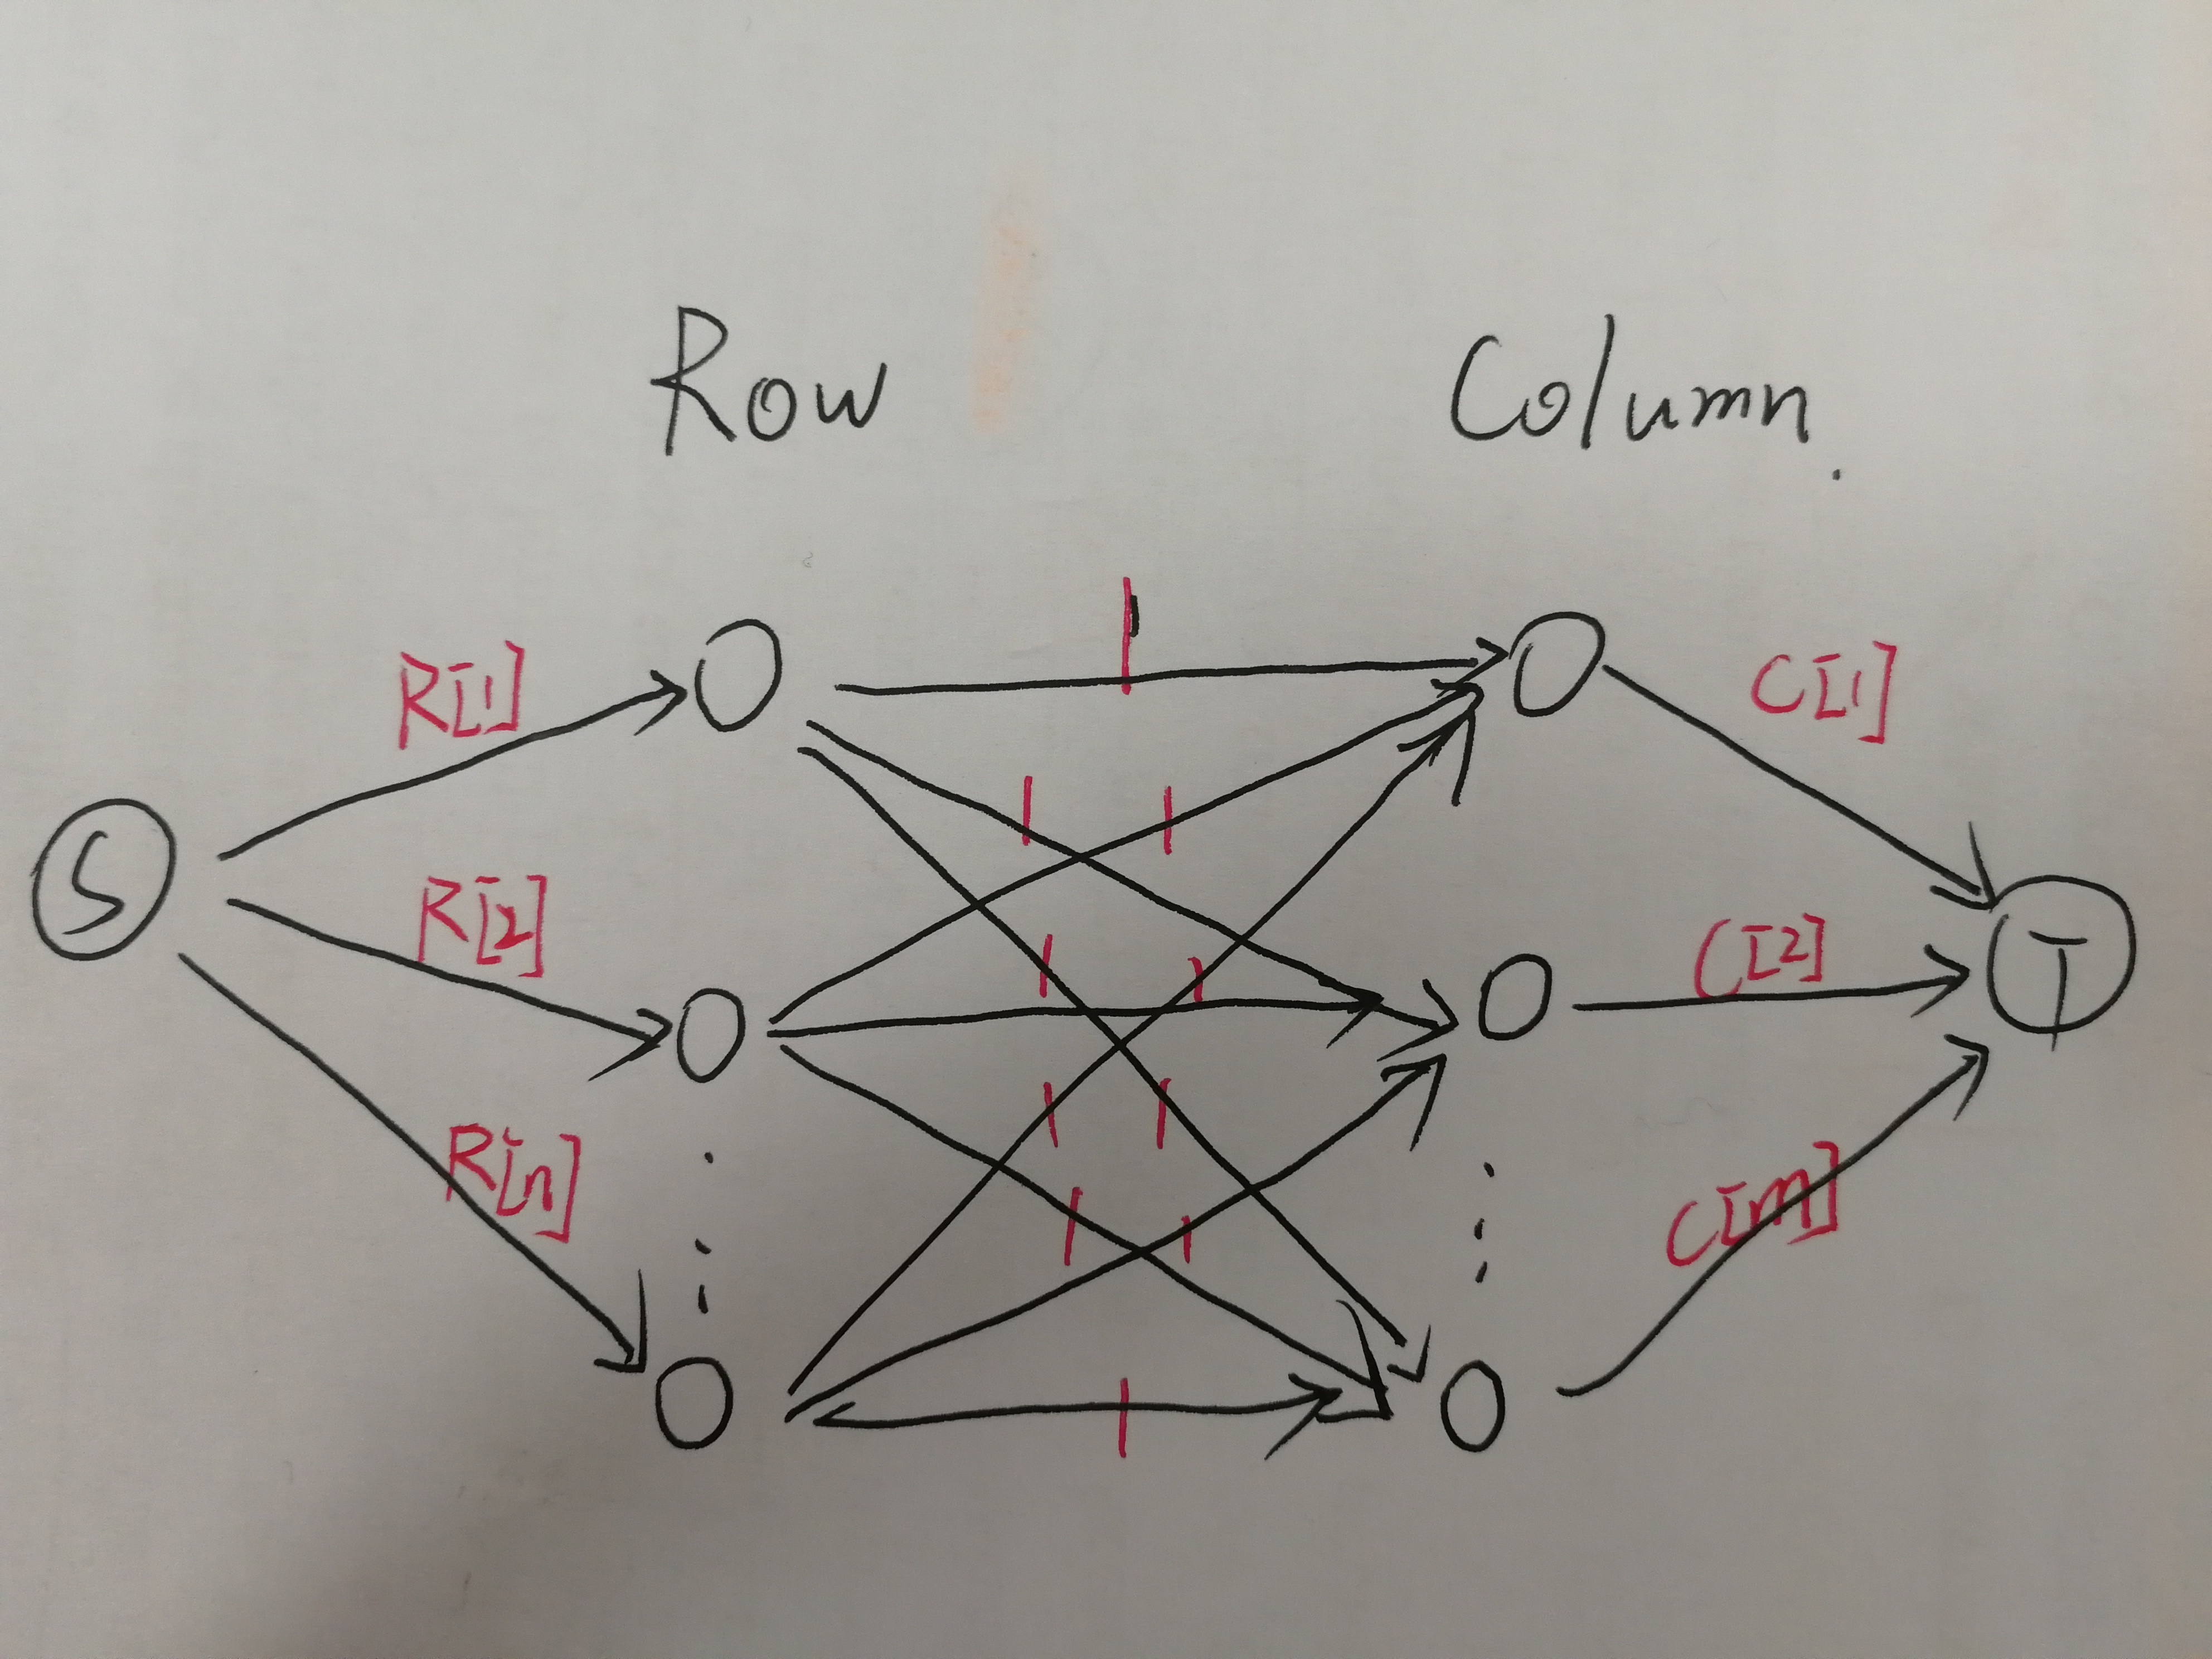
\includegraphics[scale=.1]{./2.jpg}
		\caption{Matrix}
	\end{figure}
	
	\subsection{伪代码}
	\begin{algorithm}
		\caption{Matrix}
		\begin{algorithmic}[1]
			\Require sum of each row and colum; R,C
			\Ensure Matrix
			\Function{find\_matrix}{R[n],C[m]}
				\If sum(R) != sum(C)
					\State \Return Null
				\EndIf
				\State 创建超级源点、汇点 $S,T$,构造网络流图G
				\State $f,f\_ma=Dinic(G)$执行Dinic算法,求出最大流f以及各边的流量值
				\If{$f==sum(R)$}
					\State 根据$ f\_ma $构造矩阵Matrix
					\State \Return Matrix
				\EndIf
				\State \Return Null
			\EndFunction
		\end{algorithmic}
	\end{algorithm}
	\subsection{可行性证明}
		首先我们将每行每列的总和值都转化为流量,即边的capacity,用超级源点S指向各行结点,并设置capacity为行和,这就保证了每一行的最大和不超过其设定的和值;同理,列结点指向超级汇点T也满足条件;而行结点指向各列结点的capacity,我们都设置为1,这就保证在该行该列那个位置处最多会出现一个点。
		
		然后运行Dinic算法求出最大流,如果最大流不等于总和,说明没有这样的矩阵存在;否则存在,然后获取网络流图中各个边的流量,根据行节点和列节点之间边的流量值构造矩阵,这就是最后的矩阵。所以算法正确。
		
	\subsection{时间复杂度}
	假设有n行m列。
	
	那么边的数目$ M=m+n+m*n $,节点数目$ N=1+m+n+1=m+n+2 $,运行Dinic算法的时间复杂度为$ O(N^2M) $,所以时间复杂度为:
	
	\begin{equation*}
	\begin{split}
	O(N^{2}M)
	\end{split}
	\end{equation*}
	其中:$ N=m+n+2 $、$ M=m+n+m*n $



	\newpage
	\section{Problem Reduction}
	\subsection{题目描述}
	There is a matrix with numbers which means the cost when you walk through this point. you are asked to walk through the matrix from the top left point to the right bottom point and then return to the top left point with the minimal cost. Note that when you walk from the top to the bottom you can just walk to the right or bottom point and when you return, you can just walk to the top or left point. And each point CAN NOT be walked through more than once.
	
	\subsection{解题思路}
	假设矩阵有n行m列。
	
	根据题意,从左上角的点到最右下角的点,然后再回来,使得这条回路中没有经过重复的点,我们可以将原问题转化为找出从左上角的点到最右下角的点的两条没有经过重复节点的路径。
	
	建图如下:
	
	\begin{figure}[htb]
		\centering
		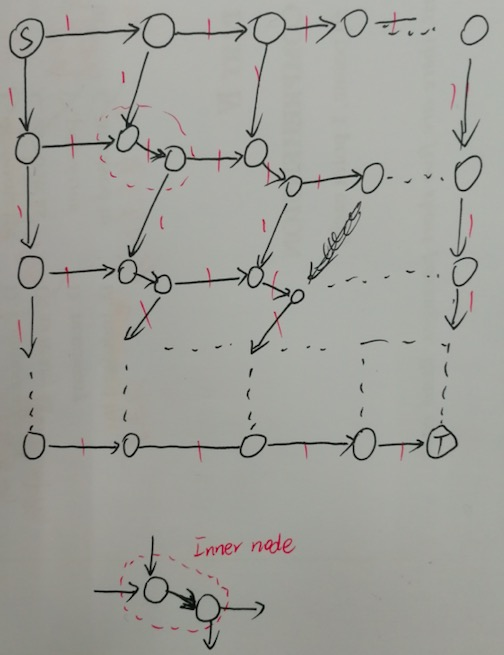
\includegraphics[scale=.6]{./4.png}
		\caption{Problem Reduction}
	\end{figure}
	
	因此,可以设置左上角的点为源点S,右下角的点为T,又因为规则说明只能向右或向下,因此,只需要将当前节点指向它右面和下面的节点以建立连边,规则要求不能经过重复的节点,那么更不可能经过同一条边,因此可以将capacity设置为1;规则要求不能就跟重复的点,我们可以将每个内部节点转化为两个节点,一个节点与左面和上面的点相连,另一个点指向右面和下面的点,设置这两个点之间的边capacity为1。然后运行Dinic算法,若最大流为2,则说明可以找到这样的两条路径。然后根据网络流图中的流量建立这样的两条路径,并将其中一条路径方向反转,这样就形成最终的解。
	

	
	\subsection{伪代码}
	\begin{algorithm}
		\caption{Problem Reduction}
		\begin{algorithmic}[1]
			\Require Matrix,M
			\Ensure Path,p
			\Function{find\_matrix}{M}
			\State 根据上面建图思路构造网络流图G
			\State $f,f\_ma=Dinic(G)$执行Dinic算法,求出最大流f以及各边的流量值
			\If{$f==2$}
			\State 根据$ f\_ma $构造两条路径$ p_1,p_2 $
			\State 反转$ p_2 $的方向,将其与$ p_1 $拼接,构造出路径$ p $
			\State \Return p
			\EndIf
			\Return Null
			\EndFunction
		\end{algorithmic}
	\end{algorithm}
	\subsection{可行性证明}
	首先每个节点只指向右面和下面的点,这就限制路径只能朝右面或下面的方向。边的capacity设置为1,这样每条边至多经过一次;对于节点,根据上面建图可直观发现内部节点被分离后的两个节点之间的capacity设为1,这样就限制了该节点最多只能经过一次。而对于外围节点,由于其左右或上下的边capacity都设置为1,它的入边总capacity和出边的总capacity必有一个为1,因此,这就限制外围节点只能经过一次,这也是不需要对其进行分离的原因。
	
	另一方面,原题要求找一个回路,我们将其转化为找两条从左上到右下的路径,因为这两条的路径的源点都为S,汇点都为T,将其中一条路径方向翻转,这样源点就变成T,汇点就变成S,拼接起来正是原题要求的路径。
	
	如果运行最大流算法能找到这样的两条路径,即最大流为2,则原问题存在解;否则,无解。
	
	\subsection{时间复杂度}
	假设有n行m列。
	
	那么边的数目$ M=(n-1)*(m-1)+ (m-2)*(n-2) = 2mn-3m-3n+5$,节点数目$ N=2*m+2*n-4+(m-2)*(n-2)*2 = 2mn-2m-2n+4 $,运行Dinic算法的时间复杂度为$ O(N^2M) $,所以时间复杂度为:
	
	\begin{equation*}
	\begin{split}
	O(N^{2}M)
	\end{split}
	\end{equation*}
	其中:$ N=2mn-2m-2n+4 $、$ M=2mn-3m-3n+5 $

	\end{CJK}	

\end{document} 
